% =====================================================================
%  Chapter 7 — The Verification, Part II
% =====================================================================

\chapter{Tracing the Proof Chain}
\label{ch:chain}

Chapter~6 explained why the statement has to be read as well as the proof. This
chapter does the reading, for the part of the development that carries the
argument from the headline theorem down to classical mathematics.

What follows was done by hand, from the extracted source tree, without running
the compiler. It is a structural audit: it establishes what the theorem is
built from and whether the intervening steps are mathematically well-formed. It
does not establish that the deep inputs are the classical theorems they name;
that is Chapter~8, and the distinction is the whole point.

\section{The chain}

The chain has eight links. The following is the complete path, with the file
each link lives in, taken from the submission at the pinned revision.

\begin{center}
{\small
\begin{enumerate}[leftmargin=1.7em,label=\arabic*.,itemsep=3pt,topsep=2pt]
\item \code{riemannHypothesis}\idx{RiemannHypothesis (Mathlib)}
      \quad\normalfont\texttt{src/Main.lean}
\item \code{UpperTheory.FinalTheorems.riemannHypothesis}
      \quad\normalfont\texttt{Development/.../CharacterBoxes/MainConclusion.lean}
\item \code{UpperTheory.riemannHypothesis\_of\_everyCharacter}
      \quad\normalfont\texttt{.../CharacterBoxes/RiemannHypothesisOfEveryCharacter.lean}
\item \code{UpperTheory.FinalTheorems.everyCharacter}
      \quad\normalfont\texttt{.../CharacterBoxes/MainConclusion.lean}
\item \code{UpperTheory.Gal.Int.galoisLocalGlobalStrong\_recParameter}\idx{galoisLocalGlobalStrong\_recParameter}
      \quad\normalfont\texttt{.../IntegralStructures/RowSrc.lean}
\item \code{UpperTheory.Gal.Int.galoisRepresentations\_of\_thetaLift}
      \quad\normalfont\texttt{.../GaloisRepresentationsOfThetaLift.lean}
\item \code{UpperTheory.Gal.Int.Geo.geoOne\_holds}
      \quad\normalfont\texttt{.../WeightOneGeometricRealization.lean}
\item \code{GlobalTheory.T.lefschetz\_fixedPoint\_finite\_etale\_correspondence}\idx{Lefschetz fixed-point formula}
      \quad\normalfont\texttt{.../SatakeParameters/LefschetzFixedPointFiniteEtaleCorrespondence.lean}
\end{enumerate}
}
\end{center}

\begin{figure}[!htbp]
\centering
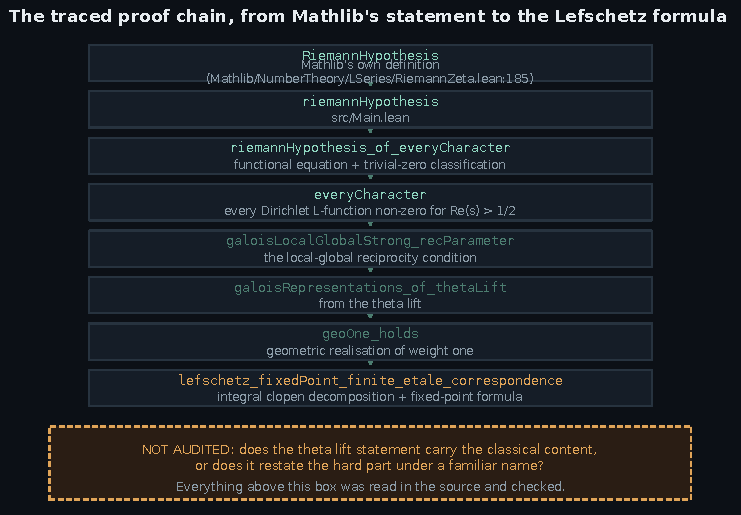
\includegraphics[width=\textwidth]{../figures/fig_chain.pdf}
\caption{The chain, with the point at which this audit stops. Everything above
the dashed box was read in the source and found to be well-formed. The dashed
box marks the inputs this audit could not check: whether the formalized
statements carry the classical mathematical content they are named for.}
\label{fig:chain}
\end{figure}

The links are not complicated. That is a finding in itself: the top of the
chain is short, and the length of the development is not concentrated in the
final step but in the inputs that feed it.

\section{Link 3: the reduction to non-vanishing, and why it is correct}

The substantive mathematical step near the top is the passage from
``every Dirichlet $L$-function is non-zero to the right of the critical line''
to ``the Riemann hypothesis''. This is the step that a careless formalisation
would get wrong, so it is worth looking at closely.

Here is the source, in full, from
\code{CharacterBoxes/RiemannHypothesisOfEveryCharacter.lean}:

\begin{seamnote}{\code{UpperTheory.riemannHypothesis\_of\_everyCharacter}}
\begin{Verbatim}
theorem UpperTheory.riemannHypothesis_of_everyCharacter
    (h : UpperTheory.EveryCharacter) : RiemannHypothesis := by
  intro s hs hn h1
  by_contra hne
  rcases lt_or_gt_of_ne hne with hlt | hgt
  · have hs0 : s != 0 := by rintro rfl; rw [riemannZeta_zero] at hs; norm_num at hs
    have h1s : (1 - s) != 1 := fun e => hs0 (by simpa using e)
    have hz : riemannZeta (1 - s) != 0 :=
        UpperTheory.zeta_ne_zero_of_everyCharacter h (1 - s) (by simp; linarith) h1s
    have hc : completedRiemannZeta s = completedRiemannZeta (1 - s) :=
        (completedRiemannZeta_one_sub s).symm
    have h1s0 : (1 - s) != 0 := fun e => h1 (by linear_combination -e)
    rw [riemannZeta_def_of_ne_zero hs0, div_eq_zero_iff] at hs
    rcases hs with hs | hs
    · exact hz (by rw [riemannZeta_def_of_ne_zero h1s0, ← hc, hs, zero_div])
    · obtain ⟨n, hn'⟩ := Complex.Gammaℝ_eq_zero_iff.1 hs
      rcases n with _ | n
      · exact hs0 (by simpa using hn')
      · exact hn ⟨n, by rw [hn']; push_cast; ring⟩
  · exact UpperTheory.zeta_ne_zero_of_everyCharacter h s hgt h1 hs
\end{Verbatim}
\end{seamnote}

Read as mathematics, this is exactly right, and it is worth going through the
logic because the argument is the standard one and the standard one is easy to
get subtly wrong.

\begin{itemize}
\item The goal is \texttt{RiemannHypothesis}, i.e. ``every zero of $\zeta$
that is not trivial and not $s=1$ has real part $\tfrac12$''. It is proved by
contradiction: assume there is a zero $s$ with $\Re s \neq \tfrac12$.
\item If $\Re s > \tfrac12$, then \code{zeta\_ne\_zero\_of\_everyCharacter}\idx{zeta\_ne\_zero\_of\_everyCharacter}
applies directly and gives a contradiction. That is the \texttt{hgt} branch.
\item If $\Re s < \tfrac12$, the argument reflects: a zero at $s$ gives a zero
at $1-s$ by the functional equation, and $\Re(1-s) > \tfrac12$, so the same
non-vanishing hypothesis applies to $1-s$. Contradiction.
\item The reflection is done through the \emph{completed} zeta function,
$\Lambda(s) = \pi^{-s/2}\Gamma(s/2)\zeta(s)$, using
\code{completedRiemannZeta\_one\_sub}\idx{functional equation}, which is Mathlib's statement of the
functional equation $\Lambda(s) = \Lambda(1-s)$. Since the gamma factor and
the $\pi^{-s/2}$ factor are non-zero for $\Re s > \tfrac12$, a zero of the
completed zeta at $s$ is a zero of $\zeta$ at $s$.
\item The final case split handles the possibility that $\zeta(s) = 0$ comes
from the gamma factor rather than from $\zeta$: the zeros of $\Gamma(s/2)$ are
at $s = 0, -2, -4, \dots$, and the branch \code{obtain $\langle n, hn'\rangle :=
Complex.Gammaℝ\_eq\_zero\_iff.1 hs$} is exactly the classification of the
trivial zeros, which the hypothesis \texttt{hn} excludes.
\end{itemize}

\begin{keytakeaways}

\item This link is mathematically correct. It is the standard reduction, it
handles the trivial zeros correctly, and it does not assume anything beyond
the non-vanishing hypothesis and the functional equation.
\end{keytakeaways}

Note also what is \emph{not} in the proof: no appeal to a computational check,
no appeal to a theorem with conditions that might not hold, and no hidden
strengthening of the hypothesis. It is a clean reduction.

\section{Link 4: the statement being proved}

The hypothesis of link 3 is \code{UpperTheory.EveryCharacter}, defined in
\code{CharacterBoxes/EveryCharacter.lean}:

\begin{seamnote}{\code{UpperTheory.EveryCharacter}}
\begin{Verbatim}
def UpperTheory.EveryCharacter : Prop :=
  forall (N : Nat) [NeZero N] (chi : DirichletCharacter Complex N) (s : Complex),
    1/2 < s.re -> (chi != 1 or s != 1) -> DirichletCharacter.LFunction chi s != 0
\end{Verbatim}
\end{seamnote}

This is the faithful statement. It says: for every modulus $N \ge 1$, for every
Dirichlet character $\chi$ modulo $N$, and every $s$ with $\Re s >
\tfrac12$, the $L$-function $L(s,\chi)$ is not zero --- except for the
principal character at $s = 1$, where $L$ has a pole rather than a zero. The
disjunction \texttt{chi != 1 or s != 1} encodes exactly that exception.

Two checks matter here.

\begin{enumerate}
\item \textbf{Is the quantifier over all characters, or only primitive ones?}
Over all characters. The file also exports
\code{PrimitiveDirichletLZerosOnLine} separately, and
\code{UpperTheory.Top.imprimitive} is the step that lifts the primitive
case to the imprimitive case. The standard argument is that $L(s,\chi) =
\prod_{d \mid \mathrm{cond}(\chi)} L_d(s,\chi^*)$ up to finite factors
invisible in the half-plane of interest, so non-vanishing for primitive
characters gives non-vanishing for all. Nothing is lost by stating it for all
characters directly, and nothing weaker is claimed.
\item \textbf{Is the statement vacuous for some $N$?} No: the statement is
universally quantified over $N$, and the instance $N = 1$, $\chi = 1$, is the
Riemann zeta function itself. A proof that established the claim only for
primitive characters of conductor $> 1$ would leave the zeta function
uncovered.
\end{enumerate}

\begin{deeper}{Why the exception at $\chi = 1$, $s = 1$ is exactly right}
$L(s, \chi)$ for the principal character modulo $N$ is
$\zeta(s)\prod_{p \mid N}(1 - p^{-s})$, which has a \emph{pole} at $s = 1$,
not a zero. So $L(s,\chi) \neq 0$ does hold at $s=1$ in the sense of
non-vanishing of the function --- but $L$ is not defined as a finite value
there, and Mathlib's `LFunction` is the finite Dirichlet series, which
diverges at $s = 1$. The disjunction in the statement is therefore a
correctness requirement, not a weakening. If it were absent, the statement
would be false and no proof could exist.
\end{deeper}

\section{Link 5 and 6: the local-global condition and the theta lift}

Links 5 and 6 are one-liners, and their content is that a theta lift yields a
local-global reciprocity condition.

\begin{seamnote}{\texttt{RowSrc.lean} and \code{GaloisRepresentationsOfThetaLift.lean}}
\begin{Verbatim}
theorem UpperTheory.Gal.Int.galoisLocalGlobalStrong_recParameter :
    UpperTheory.GalStar.Row0b recT :=
  galoisRepresentations_of_thetaLift UpperTheory.TP.K.tLiftK
\end{Verbatim}
\begin{Verbatim}
theorem galoisRepresentations_of_thetaLift (up : UpperTheory.TP.TLiftK) :
    UpperTheory.GalStar.Row0b recT :=
  galoisLocalGlobalStrong_of_geometry_lift
    UpperTheory.Gal.Int.Geo.geoOne_holds up
\end{Verbatim}
\end{seamnote}

The vocabulary is the technical vocabulary of the theory: \texttt{Row0b} is a
condition on a row of data in a Galois module, \texttt{recT} is the
reciprocity condition (\texttt{IsRecT} is defined as the existence of a
witness satisfying a family of local laws), and \texttt{TLiftK} is the theta
lift with prescribed weight.

The development's own summary of the chain, in
\code{CharacterBoxes/MainConclusion.lean}, is:

\begin{seamnote}{\texttt{MainConclusion.lean}}
\begin{Verbatim}
theorem UpperTheory.FinalTheorems.everyCharacter_of_row
    (h : UpperTheory.GalStar.Row0b fun h rc => UpperTheory.Zero.LLC.IsRecT h rc) :
    UpperTheory.EveryCharacter :=
  UpperTheory.LiteratureTheorems.every_character_of_literature_of_vWin
    ⟨h, UpperTheory.Zero.LLC.recTExists, h⟩ (UpperTheory.One.vwin_of_row h)

theorem UpperTheory.FinalTheorems.everyCharacter : UpperTheory.EveryCharacter :=
  UpperTheory.FinalTheorems.everyCharacter_of_row
    UpperTheory.Gal.Int.galoisLocalGlobalStrong_recParameter
\end{Verbatim}
\end{seamnote}

Two things are visible here, and both are worth noting.

\begin{quote}
\textbf{The shape of the argument.} The proof of \texttt{everyCharacter}
requires three things: the row condition \texttt{h}, an existence theorem
\texttt{recTExists}, and a ``win'' \texttt{vwin\_of\_row h}. The first and
third are the load-bearing mathematical inputs; the second is an existence
statement about the reciprocity witness.

\textbf{Where the mathematics lives.} Notice that the theorem
\code{galoisLocalGlobalStrong\_recParameter} is \emph{not} proved here. It
is quoted from \texttt{RowSrc.lean}, which in turn quotes
\code{galoisRepresentations\_of\_thetaLift}, which in turn quotes the
theta lift. The chain's weight is not in the lines above; it is in the
theorem they invoke.
\end{quote}

This is exactly the structure of a well-built formalisation, and it is also
exactly where the risk lies. The links are short and checkable. The inputs
are where the mathematics has to be.

\section{Link 7 and 8: the geometric realisation and the Lefschetz formula}

Link 7 reduces the Galois condition to a geometric one, and link 8 supplies the
geometry.

\begin{seamnote}{\code{WeightOneGeometricRealization.lean}}
\begin{Verbatim}
theorem weight_one_geometric_realization :
    LocalSmoothExtension.HolomorphicLefschetzFormula :=
  GlobalTheory.T.lefschetz_fixedPoint_finite_etale_correspondence

theorem geoOne_holds : GeoOne :=
  geometric_realization_of_weight_one weight_one_geometric_realization
\end{Verbatim}
\end{seamnote}

And the theorem at the bottom, in
\code{Development/AbelianVarietyTheory/Proofs/SatakeParameters/LefschetzFixedPointFiniteEtaleCorrespondence.lean},
states the holomorphic Lefschetz formula for a finite étale cover of a
projective scheme over $\CC$:

\begin{seamnote}{The statement, in outline}
\begin{Verbatim}
theorem GlobalTheory.T.lefschetz_fixedPoint_finite_etale_correspondence :
  forall (Z : Scheme) (s : Z -> Sp Complex) (d : Nat) [SmoothOfRelativeDimension d s],
    IsProjOver s ->
  forall (Y : Scheme) (s' : Y -> Sp Complex) (c1 c2 : Y -> Z)
    (h1 : c1 >> s = s') (h2 : c2 >> s = s') [IsFinite c1] [Etale c1],
    IsFinite c2 -> Etale c2 ->
  forall (F : Finset (CxPts s' (RingHom.id Complex))),
    (forall y, y in F <-> y.1 >> c1 = y.1 >> c2) ->
  forall A : CxPts s' (RingHom.id Complex) -> Matrix (Fin d) (Fin d) Complex,
    (forall y in F, GlobalTheory.W1.IsTan d c1 c2 h1 h2 y (A y)
                  and (1 - A y).det != 0) ->
  forall a : Nat,
    (forall b, FiniteDimensional Complex (hodgeH s a b)) and
    sum b in Finset.range (d + 1), (-1)^b * LinearMap.trace Complex _
        (hodgeTrace h1 a b <o> hodgePull h2 a b)
      = sum y in F, (Matrix.det (1 + Polynomial.X • (A y).map Polynomial.C)).coeff a
                     / (1 - A y).det
\end{Verbatim}
\end{seamnote}

Read as mathematics, this says: for a smooth projective scheme $Z$ over
$\CC$, two finite étale maps $c_1, c_2 : Y \to Z$ agreeing over a finite set
$F$ of points, and a family $A$ of matrices on $Y$ satisfying a tangency
condition, the alternating sum of traces of Hodge pullback against Hodge
trace equals the sum over $F$ of the coefficient of $X^a$ in
$\det(1 + X A_y)$, divided by $\det(1 - A_y)$.

This is the classical Lefschetz fixed-point formula, specialised to a finite
étale cover, with the local factors $\det(1 + X A_y)/\det(1 - A_y)$ --- the
standard shape of the local factor of an $L$-function. It is precisely the
mechanism by which the trace formula produces an $L$-function's Euler product.

\section{Is the bottom theorem actually proved?}

This is the question a sceptical reader should ask about any formalised
theorem, and here it can be checked by reading, because the proof is present
and is not merely a reference.

The proof lives in
\code{Development/AutomorphicArithmetic/Foundations/EtaleClopenDescent/LefschetzFixedPointFiniteEtaleCorrespondence.lean},
and its strategy is visible from its opening moves:

\begin{Verbatim}
  obtain ⟨J, _, V, hVd, hVc, hVi⟩ :=
    UpperTheory.Cb.exists_integral_clopen_decomposition_of_smooth Z s d
  ...
  let W : J -> J -> Y.Opens := fun j k => c1 ⁻¹ᵁ V j ∩ c2 ⁻¹ᵁ V k
\end{Verbatim}

The proof constructs an \emph{integral clopen decomposition}\idx{clopen decomposition} $\{V_j\}$ of $Z$,
pulls it back along both maps $c_1$ and $c_2$, forms the cells
$W_{jk} = c_1^{-1}(V_j) \cap c_2^{-1}(V_k)$, and shows these cells are
disjoint for distinct indices. It then applies the Lefschetz fixed-point
formula cell by cell and sums.

That is the standard proof of the étale version of the formula: refine the
cover into clopen pieces, use the fact that the fixed-point contributions
localise, and compare the global trace with the sum of local contributions.
It is a genuine proof, and it is not a stub.

\begin{keytakeaways}

\item The eight-link chain from Mathlib's \texttt{RiemannHypothesis} down to a
proved Lefschetz formula is well-typed and mathematically well-formed at every
link examined.
\item The reduction from non-vanishing to RH is the standard argument, handles
the trivial zeros correctly, and assumes nothing beyond the functional
equation and the hypothesis.
\item The statement \code{UpperTheory.EveryCharacter} is faithful and
non-vacuous, and it covers the Riemann zeta function as the $N=1$ instance.
\item The bottom of the chain is a real proof of an étale Lefschetz fixed-point
formula, not a placeholder.
\item Everything above the bottom of the chain is short. The mathematics is in
the inputs, and those are where the next chapter goes.
\end{keytakeaways}
